\documentclass[]{article}
\usepackage{lmodern}
\usepackage{amssymb,amsmath}
\usepackage{ifxetex,ifluatex}
\usepackage{fixltx2e} % provides \textsubscript
\ifnum 0\ifxetex 1\fi\ifluatex 1\fi=0 % if pdftex
  \usepackage[T1]{fontenc}
  \usepackage[utf8]{inputenc}
\else % if luatex or xelatex
  \ifxetex
    \usepackage{mathspec}
  \else
    \usepackage{fontspec}
  \fi
  \defaultfontfeatures{Ligatures=TeX,Scale=MatchLowercase}
\fi
% use upquote if available, for straight quotes in verbatim environments
\IfFileExists{upquote.sty}{\usepackage{upquote}}{}
% use microtype if available
\IfFileExists{microtype.sty}{%
\usepackage{microtype}
\UseMicrotypeSet[protrusion]{basicmath} % disable protrusion for tt fonts
}{}
\usepackage[margin=1in]{geometry}
\usepackage{hyperref}
\hypersetup{unicode=true,
            pdftitle={Analyzing DECREASE trials to estimate evidence of data manipulation},
            pdfauthor={Chris HJ Hartgerink, Gerben ter Riet, Marleen Kemper, Markus Hollman},
            pdfborder={0 0 0},
            breaklinks=true}
\urlstyle{same}  % don't use monospace font for urls
\usepackage{longtable,booktabs}
\usepackage{graphicx,grffile}
\makeatletter
\def\maxwidth{\ifdim\Gin@nat@width>\linewidth\linewidth\else\Gin@nat@width\fi}
\def\maxheight{\ifdim\Gin@nat@height>\textheight\textheight\else\Gin@nat@height\fi}
\makeatother
% Scale images if necessary, so that they will not overflow the page
% margins by default, and it is still possible to overwrite the defaults
% using explicit options in \includegraphics[width, height, ...]{}
\setkeys{Gin}{width=\maxwidth,height=\maxheight,keepaspectratio}
\IfFileExists{parskip.sty}{%
\usepackage{parskip}
}{% else
\setlength{\parindent}{0pt}
\setlength{\parskip}{6pt plus 2pt minus 1pt}
}
\setlength{\emergencystretch}{3em}  % prevent overfull lines
\providecommand{\tightlist}{%
  \setlength{\itemsep}{0pt}\setlength{\parskip}{0pt}}
\setcounter{secnumdepth}{0}
% Redefines (sub)paragraphs to behave more like sections
\ifx\paragraph\undefined\else
\let\oldparagraph\paragraph
\renewcommand{\paragraph}[1]{\oldparagraph{#1}\mbox{}}
\fi
\ifx\subparagraph\undefined\else
\let\oldsubparagraph\subparagraph
\renewcommand{\subparagraph}[1]{\oldsubparagraph{#1}\mbox{}}
\fi

%%% Use protect on footnotes to avoid problems with footnotes in titles
\let\rmarkdownfootnote\footnote%
\def\footnote{\protect\rmarkdownfootnote}

%%% Change title format to be more compact
\usepackage{titling}

% Create subtitle command for use in maketitle
\newcommand{\subtitle}[1]{
  \posttitle{
    \begin{center}\large#1\end{center}
    }
}

\setlength{\droptitle}{-2em}
  \title{Analyzing DECREASE trials to estimate evidence of data manipulation}
  \pretitle{\vspace{\droptitle}\centering\huge}
  \posttitle{\par}
  \author{Chris HJ Hartgerink, Gerben ter Riet, Marleen Kemper, Markus Hollman}
  \preauthor{\centering\large\emph}
  \postauthor{\par}
  \predate{\centering\large\emph}
  \postdate{\par}
  \date{14 July, 2017}


\begin{document}
\maketitle

The effect of beta-blockers on perioperative mortality in non-cardiac
surgery has been controversial\textsuperscript{1} due to concerns
regarding the scientific integrity in two related clinical
trials\textsuperscript{2--6}. Three meta-analyses that included the
trials subject to concerns concluded that beta-blockers decrease
perioperative mortality\textsuperscript{7--9} whereas a meta-analysis
that excluded the suspect trials concluded that beta-blockers increase
perioperative mortality\textsuperscript{9}. In these studies,
perioperative mortality was defined as the death rate of patients in the
perioperative setting, including the period of admission, anaesthesia
with surgery, and postoperative recovery.

The trials subject to concerns regarding scientific integrity were the
Dutch DECREASE-I and DECREASE-IV trials\textsuperscript{4--6}. The
committees that investigated the integrity of the DECREASE trials
reported that data manipulation was likely but that the extent of the
data manipulation remained unclear\textsuperscript{4--6}. Moreover, the
latest guidelines still recommend the usage of beta-blockers in the
perioperative period in certain cases\textsuperscript{10,11}, where some
of these guidelines are based on other work by the PI of the DECREASE
trials. Considering the potential harmful consequences of guidelines
based on work by someone who has been repeatedly investigated for
breaching scientific integrity, we aim to estimate the extent of data
manipulation in the DECREASE studies\textsuperscript{2--6} to further
stimulate the debate on using beta-blockers in the perioperative period
patients undergoing non-cardiac surgery.

The reports on the integrity of the DECREASE trials primarily focused on
the provenance of the raw data but did not investigate the extent to
which the DECREASE trials deviated from comparable trials. Provenance is
primarily concerned with the origins of the data, verifying things such
as (but not limited to) the informed consent and whether data
corresponded to patient files. The committee reports did not neglect
statistical evaluation however: according to the report a statistical
expert evaluated the applicability of forensic statistical
methods\textsuperscript{6} to evaluate results of trials separately
(i.e., DECREASE-I, DECREASE-IV) although it lacks details as to how this
evaluation took place. The expert concluded that the previously applied
methods by him were not applicable for use in this case. Nonetheless, in
this report we compare across trials, which is a method that has
previously been used to monitor trial data quality or to test for
potential data anomalies\textsuperscript{12,13}. Moreover, comparing
across trials instead of evaluating them separately has previously
proven to be effective in detecting data
manipulation\textsuperscript{14}. Comparing the DECREASE trials to other
published trials studying the effectiveness of beta-blockers with
respect to perioperative mortality could prove informative of the
potential extent of the manipulation in the DECREASE trials.

The effectiveness of perioperative beta-blockade is obfuscated by the
afflicted DECREASE trials, potentially interacting with the type of
beta-blocker and the way that beta-blockers were administered (i.e.,
dose and duration of treatment). In the randomized trials on
beta-blockers, patients were administered various types of beta-blockers
(e.g., metroprolol, bisoprolol, atenolol) and in various ways (e.g.,
intravenously, orally; half an hour before surgery or multiple days
before surgery; with or without titration based on heart rate). Factors
such as dosage and duration can have an effect on the pharmacological
effectiveness with respect to perioperative mortality. Moreover, the
highly discrepant results from the DECREASE trials\textsuperscript{9}
might partly be caused by such differences\textsuperscript{15} and not
purely due to data manipulation (given that not all data points can be
considered manipulated at this point).

To statistically investigate the evidence for data manipulation in the
DECREASE studies\textsuperscript{2,3}, we took three steps. First, we
reproduced the findings from the 2014 meta-analysis by Bouri et
al.\textsuperscript{9}, which contained sufficient information to
estimate the deviation of the DECREASE trials from other published
trials on beta-blockers. We also included type of beta-blocker to
inspect whether this is predictive of the effect of beta-blockers on
perioperative mortality. Second, we evaluated the probability that the
DECREASE trials occurred assuming no data manipulation. Third, we
reversed this assumption and assumed that data manipulation did occur
and estimated how many data points would have to be manipulated in order
to reproduce the results of the DECREASE trials, if the other published
trials are regarded as estimating the true effect of beta-blockers on
perioperative mortality in patients undergoing non-cardiac surgery.
Considering the committees investigating the scientific integrity of the
DECREASE trials was unable to assess this, we consider it worthwhile to
investigate this further.

\subsection{Step 1: reproducing meta-analysis of Bouri et al.
(2014)}\label{step-1-reproducing-meta-analysis-of-bouri-et-al.-2014}

\subsubsection{Methods}\label{methods}

To ensure that we used similar analysis procedures as in the 2014
meta-analysis\textsuperscript{9}, we initially reproduced Bouri et al.'s
estimates. This ensured that (1) their results are reproducible and (2)
we are using the correct estimates in subsequent steps of our analyses.
Using figures 2 and 3 from the original paper\textsuperscript{9}, we
extracted the raw event data for the 2 (control vs experimental) by 2
(event vs no event) design, which we used to recompute the natural
logarithm of the risk ratio and its standard error. The extracted event
data is available at \href{https://osf.io/aykeh}{osf.io/aykeh} and our
analysis plan was preregistered at
\href{https://osf.io/vnmzc}{osf.io/vnmzc}.

We computed the log risk ratio (i.e., log RR) for each study and pooled
these using the \texttt{R} package \texttt{metafor}\textsuperscript{16}.
We estimated a weighted random-effects model using the restricted
maximum-likelihood estimator (i.e., \texttt{REML})\textsuperscript{17}
to estimate the variance of effects. We used the default weighting
procedure in the \texttt{metafor} package. We added 0.5 to each cell
count, as is common in meta-analyses on risk- and odds ratios in order
to prevent computational artefacts {[}18; p397{]}. The 2014
meta-analysis\textsuperscript{9} did not specify the variance estimate
used; hence, minor discrepancies between our estimates and the original
estimates could be due to differences in the estimation procedure.

\subsubsection{Results}\label{results}

We were able to closely reproduce the estimates for the different sets
of studies (Figure 2 of the 2014 meta-analysis\textsuperscript{9}).
Bouri et al. differentiated between the estimates from the non-DECREASE
trials (\(k=9\)) and the DECREASE trials (\(k=2\)). We confirmed the
effect size estimates and the variance estimates for both the
non-DECREASE- and the DECREASE trials, except for some minor
discrepancies at the second decimal level. Table 1 depicts the original
and reproduced values for both sets of studies.

\begin{longtable}[]{@{}lllll@{}}
\caption{The original- and reproduced meta-analytic results based on the
data provided in the 2014 meta-analysis by Bouri et al.}\tabularnewline
\toprule
& & Risk ratio & \(\tau^2\) & Confidence interval\tabularnewline
Non-DECREASE (k=9) & Original & 1.27 & 0 & {[}1.01;
1.60{]}\tabularnewline
& Reproduced & 1.27 & 0 & {[}1.01; 1.61{]}\tabularnewline
DECREASE (k=2) & Original & 0.42 & 0.29 & {[}0.15;
1.23{]}\tabularnewline
& Reproduced & 0.47 & 0.14 & {[}0.19; 1.15{]}\tabularnewline
\bottomrule
\end{longtable}

Second, we meta-analyzed all studies combined, including a dummy
predictor for the DECREASE and non-DECREASE studies to reproduce results
presented in Figure 4 of the 2014 meta-analysis\textsuperscript{9}.
Surprisingly, our results showed a bit more evidence against equal
subgroups than the original meta-analysis\textsuperscript{9} (original:
\(\chi^2(1)=3.91,p=.05\); reproduced: \(\chi^2(1)=6.12,p=0.013\)).
Additionally, the original analyses showed substantial residual
heterogeneity (\(I^2=74.4\)\%) whereas we found no residual
heterogeneity (\(I^2=0\)\%). Different variance estimates (e.g.,
\texttt{DerSimonian-Laird} instead of \texttt{REML}) did not resolve
this difference. We tried to clarify these discrepancies by e-mailing
the original authors (including a reminder after several weeks) but did
not receive a response. Nonetheless, the broad strokes of the
meta-regression confirmed that the DECREASE trials were the determining
predictor for the effectiveness of beta-blockers (including DECREASE:
\(RR=0.509\); excluding DECREASE: \(RR=1.275\)).

Additionally, and exploratively, we evaluated the predictive effect of
the type of beta-blocker used in the trials. The DECREASE trials
remained predictive of decreased mortality (\(RR=0.509\)), whereas the
non-DECREASE trials provide tentative, but uncertain, evidence that
atenolol results in lower mortality (\(RR=0.777\)). Nonetheless, for
other beta-blockers in the non-DECREASE trials, there is still tentative
and uncertain evidence that beta-blockers increase mortality
(bisoprolol: \(RR=2.973\); metoprolol: \(RR=1.303\); propranolol:
\(RR=1.7\)). Table 2 shows the meta-regression results in full.

\begin{longtable}[]{@{}lll@{}}
\caption{Meta-regression results (k=11) for log(RR), including dummy
predictors for DECREASE trials (reference: non-DECREASE trials) and type
of beta-blockers used in the trial (reference:
atenolol).}\tabularnewline
\toprule
& Estimate & 95\% CI\tabularnewline
Intercept & -0.252 & -1.228; 0.724\tabularnewline
Non-DECREASE & - & -\tabularnewline
DECREASE & -1.765 & -5.05; 1.519\tabularnewline
Atenolol & - & -\tabularnewline
Bisoprolol & 1.342 & -2.015; 4.698\tabularnewline
Metoprolol & 0.517 & -0.49; 1.523\tabularnewline
Propranolol & 0.783 & -1.5; 3.065\tabularnewline
\bottomrule
\end{longtable}

\subsection{Step 2: evaluating the veracity of DECREASE
studies}\label{step-2-evaluating-the-veracity-of-decrease-studies}

Based on the non-DECREASE estimates from Step 1, we estimated the
probability of obtaining the results in the DECREASE trials. To this
end, we assumed that the non-DECREASE trials provide a valid
representation of the true effect of beta-blockers on perioperative
mortality (similar to Bouri et al.\textsuperscript{9}). The estimated
probability of the observed data under a given true effect is also known
as the veracity of the data\textsuperscript{19}. We assumed that the
non-DECREASE studies estimated the true effect distribution of
perioperative beta-blockade on mortality, not perturbed by publication
bias due to statistical (non)significance. Publication bias was assumed
to not be a problem because a substantial number of nonsignificant
effects are included in the dataset (9 of 11 results are
nonsignificant).

\subsubsection{Method}\label{method}

Based on the estimated mean log RR and its credible interval in the
non-DECREASE studies, we computed the probability of the observed log RR
in the DECREASE trials. The estimates of the non-DECREASE studies were
obtained from Step 1, which include the estimated log RR (i.e., 0.24),
and its 95\% credibility interval as provided by the package
\texttt{metafor} (i.e., {[}0.008; 0.477{]}). The meta-analysis model
assumes a normal distribution of population effects with the estimated
effect as the mean of the distribution. The 95\% credibility interval
denotes the bounds of the normal distribution that covers 95\% of the
density, where the standard deviation is calculated as the distance from
the mean to either bound, divided by 1.96. This allows for an
approximation of the population effect distribution, as depicted in
Figure 1.

\begin{figure}

{\centering 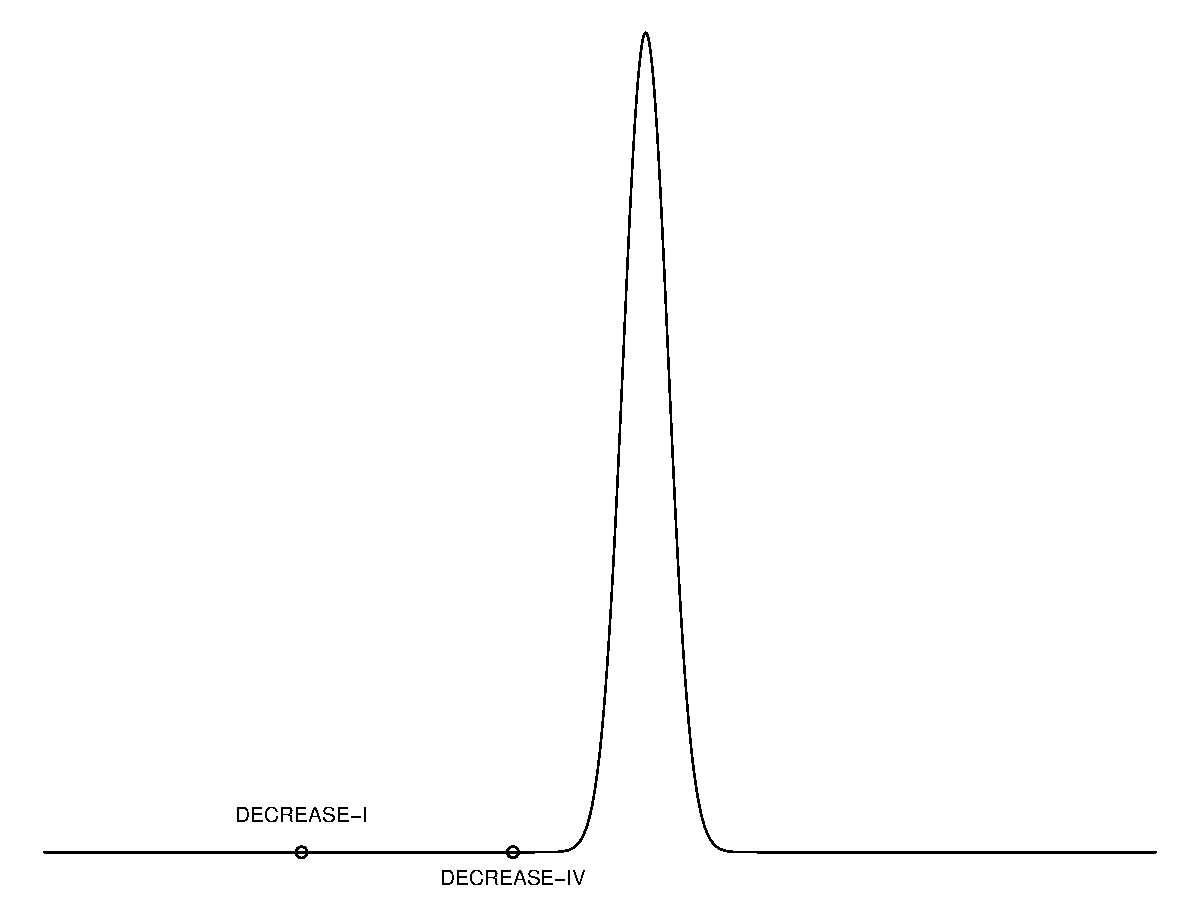
\includegraphics[width=0.8\linewidth]{../figures/fig1} 

}

\caption{Density plot of the estimated true effect distribution based on the non-DECREASE studies only, with the position of the DECREASE studies highlighted.}\label{fig:figure 1}
\end{figure}

Based on the estimated effect distribution from the non-DECREASE trials,
we calculated the probability of each DECREASE trial result, or a more
extreme result. In other words, we computed the \(p\)-value for the null
hypothesis that the DECREASE trials arise from the same effect
distribution as the non-DECREASE trials. This assumes that the
information available from the other trials is informative of the true
population effect.

\subsubsection{Results}\label{results-1}

Figure 2 indicates that the DECREASE trials are highly unlikely under
the estimated effect distribution based on the non-DECREASE trials. More
specifically, the results from DECREASE-I (or more extreme) have a
probability of \(6.9621238\times 10^{-45}\) (approximately 7 in a
\href{https://en.wikipedia.org/wiki/Names_of_large_numbers}{quattuordecillion};
\(z=-14.057\)) and the results from DECREASE-IV have a probability of
\(6.556057\times 10^{-9}\) (approximately 7 in a billion; \(z=-5.802\)).
This indicates that the DECREASE trial results are unlikely to have come
from the same population effect distribution as the non-DECREASE trials.
Moreover, observing two of such extremely unlikely results jointly, as
in the DECREASE trials, is nearly impossible,
\(4.564408\times 10^{-53}\). Hence, this result indicates that the
DECREASE trials are severely different from the non-DECREASE trials.

Results from Step 1 indicated that no between-trial variance (i.e.,
homogeneity; \(\tau^2=0\)) of the effects was observed; given the small
number of trials included (i.e., 9) this estimate is highly uncertain,
however. The total \(N\) across the non-DECREASE trials was 10529.We
conducted sensitivity analyses to see how dependent results are on the
heterogeneity estimate (not preregistered;
\href{https://osf.io/vnmzc}{osf.io/vnmzc}). The probability of observing
the DECREASE trials stays approximately below 1 out of 1000 until the
variance estimate is 0.25; the probability stays approximately below 1
out of 100 until the variance estimate is 0.43 (see Figure 2). To put
these numbers into context, a variance of 0.25 would suggest that
results of perioperative beta-blockade vary substantially due to
contextual circumstances of the study, even if perioperative
beta-blockade has no effect whatsoever (RRs between 0.779 and 1.284 in
\textasciitilde{}64\% of the cases).

\begin{figure}

{\centering 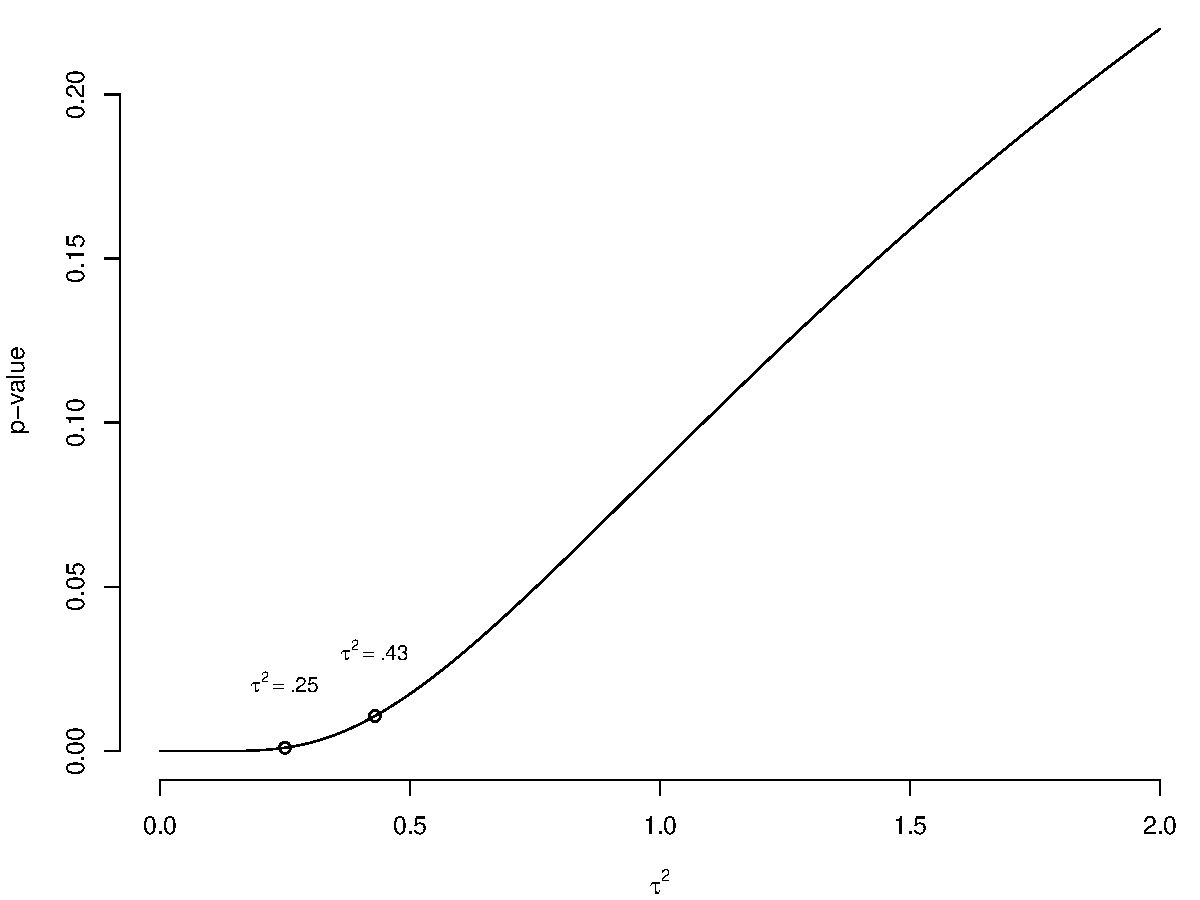
\includegraphics[width=0.8\linewidth]{../figures/fig2} 

}

\caption{Sensitivity analyses for the p-value that indicates the probability of observing the results from the DECREASE studies, or more extreme results, based on the estimated true effect (non-DECREASE trials) and the accompanying variance estimate.}\label{fig:figure 2}
\end{figure}

\subsection{Step 3: estimating the amount of manipulated
data}\label{step-3-estimating-the-amount-of-manipulated-data}

We estimated the number of data points that would need to be manipulated
to arrive at the estimates from the DECREASE trials, given that the
non-DECREASE trials represent the true effect of perioperative
beta-blockade. In contrast to Step 2, which assumes no data manipulation
occurred, Step 3 assumes that the DECREASE trials might in fact contain
manipulated data. The estimates from Step 3 provide an indication of the
extent of potential data manipulation in the DECREASE
studies\textsuperscript{4--6,9}.

\subsubsection{Method}\label{method-1}

In order to estimate the number of manipulated data points, we first
estimated the probability of perioperative mortality (in log odds) in
each trial arm for each trail stratum. As such, we estimate mortality
odds four times: once per condition (beta-blocker or control) per trial
type (DECREASE- and non-DECREASE trials). For all combinations of
condition and trial type, we ran a meta-analysis applying similar
methods used in Step 1, resulting in four meta-analytic absolute
mortality estimates with corresponding effect variances (see Table 3;
one estimate per cell). Throughout the simulations, we used the point
estimates (i.e., fixed effect) to simulate genuine- and manipulated
data, but supplemented this by using the more uncertain distribution
estimates (i.e., random effects) as sensitivity analyses.

\begin{longtable}[]{@{}lll@{}}
\caption{Outcome possibilities within a simulated 2 (beta-blocker v
control) by 2 (dead v alive) clinical trial.}\tabularnewline
\toprule
& Dead & Alive\tabularnewline
Beta-blockers & \(n_{11}\) & \(n_{12}\)\tabularnewline
Control & \(n_{21}\) & \(n_{22}\)\tabularnewline
\bottomrule
\end{longtable}

We applied the inversion method to estimate the number of manipulated
data points in the DECREASE trials\textsuperscript{20}. The inversion
method iteratively hypothesizes that \emph{X} out of \emph{N} data
points were manipulated (i.e., \(X={0, 1, ..., N}\)). For each
combination of \emph{X} and trial, we simulated 10000 datasets. Each
simulated dataset contained \emph{X} manipulated data points and
\emph{N-X} genuine data points. For each simulated dataset (exact
simulation procedure in the next paragraph), we determined the
likelihood of the results with

\begin{equation}
\label{eq1}
L(\theta|\pi_{E},\pi_{C})=\pi_{E}^{n_{11}}(1-\pi_{E})^{n_{12}} \times \pi_{C}^{n_{21}}(1 - \pi_{C})^{n_{22}}
\end{equation}

where \(\pi_{E}\) indicates the mortality rate in the beta-blocker
condition as drawn from the meta-analytic effect distribution
(\(\pi_{C}\) indicates the mortality rate in the control condition). We
estimated those parameters using the meta-analytic procedure described
in the previous paragraph, resulting in the estimates depicted in Table
4. The likelihood was computed under both the manipulated effect
estimates (i.e., \(L_{manipulated}\)) and the genuine data (i.e.,
\(L_{genuine}\)). Table 3 indicates which cell sizes the various
\(n_{XX}\) refer to within the (simulated) data. After computing the
likelihoods, we compared them to determine whether the simulated data
were more likely to arise from the genuine trials
(\(L_{genuine}>L_{manipulated}\)) or from the manipulated trials
(\(L_{manipulated}>L_{genuine}\)). Note that comparing the likelihoods
is a minor deviation from the preregistration, where we initially
planned on using \(p\)-value comparisons
(\href{https://osf.io/vnmzc}{osf.io/vnmzc}).

\begin{longtable}[]{@{}llll@{}}
\caption{Mortality estimates per condition, per trial stratum. We used
these parameters to estimate the number of manipulated data points with
the inversion method.}\tabularnewline
\toprule
& & log(odds) & \(\tau\)\tabularnewline
DECREASE (k=2) & Beta-blocker & -3.629 & 0.588\tabularnewline
& Control & -2.498 & 1.644\tabularnewline
Non-DECREASE (k=9) & Beta-blocker & -3.034 & 0.712\tabularnewline
& Control & -3.208 & 1.001\tabularnewline
\bottomrule
\end{longtable}

For each hypothesis of \emph{X} out of \emph{N} manipulated data points,
we computed the probability that the manipulated data are more likely
than the genuine data (\(p_M=P(L_{manipulated}>L_{genuine})\)). Based on
\(p_M\), we computed the confidence interval for the estimated \(X\)
manipulated data points (i.e., \(X_{LB};X_{UB}\)). For a 95\% confidence
interval, the lower bound is equal to the \(p_M\) closest to .025,
whereas the upperbound is equal to the \(p_M\) closest to .975.

We computed \(p_M\) for all \emph{X} out of \emph{N} manipulated data
points in 10000 randomly generated datasets, which were generated in
three steps. For each dataset we:

\begin{enumerate}
\def\labelenumi{\arabic{enumi}.}
\item
  Sampled (across conditions, without replacement) \emph{X} fictitious
  participants that would be the result of data manipulation.
\item
  Determined the population mortality rate for each condition (i.e., for
  each cell as in Table 3). The meta-analytic point estimate was used or
  a population effect was randomly drawn from the meta-analytic effect
  distribution.
\item
  Simulated the number of deaths for the different conditions using a
  binomial distribution based on the mortality rate as determined in 2,
  resulting in the cell counts as in Table 3.
\end{enumerate}

Based on the meta-analytic effect from 2 and the cell sizes from 3, we
computed the likelihoods \(L_{manipulated}\) and \(L_{genuine}\) using
Equation \ref{eq1}. As mentioned before, we computed \(p_M\), which
indicates the probability that the data are more likely under the
estimates resulting from the (allegedly) manipulated data (i.e., the
DECREASE trials) than under the estimates resulting from the genuine
data (i.e., the non-DECREASE trials;
\(p_M=P(L_{manipulated}>L_{genuine})\)).

\subsubsection{Results}\label{results-2}

For DECREASE-I (\(N=112\)), the 95\% confidence interval for the
estimated number of manipulated data points is {[}0 - 112{]} or {[}0 -
112{]} when based on a point estimate or a more uncertain distribution
estimate, respectively. The left column of Figure 3 depicts the \(p_M\)
per \emph{X} manipulated data points (top panel) and the bounds of the
confidence interval when the degree of confidence is altered (lower
panel). Staying clearly between the dotted lines in the top panel,
depicting the 95\% CI (top: .975; bottom: .025), it becomes apparent
that the degree of uncertainty is too high to make any reasonable
estimates about the number of manipulated data points with sufficient
confidence. This is partly due to the small sample size of the
DECREASE-I trial (i.e., \(N=112\)) and the availability of just the
summary results. Only when the degree of confidence is lowered to around
75\% does the interval not span the entire sample size. As such, based
on the summary results, little can be said about the extent of the data
manipulation that occurred in the DECREASE-I trial, affirming the
conclusions of the original committee report\textsuperscript{6}.

\begin{figure}

{\centering 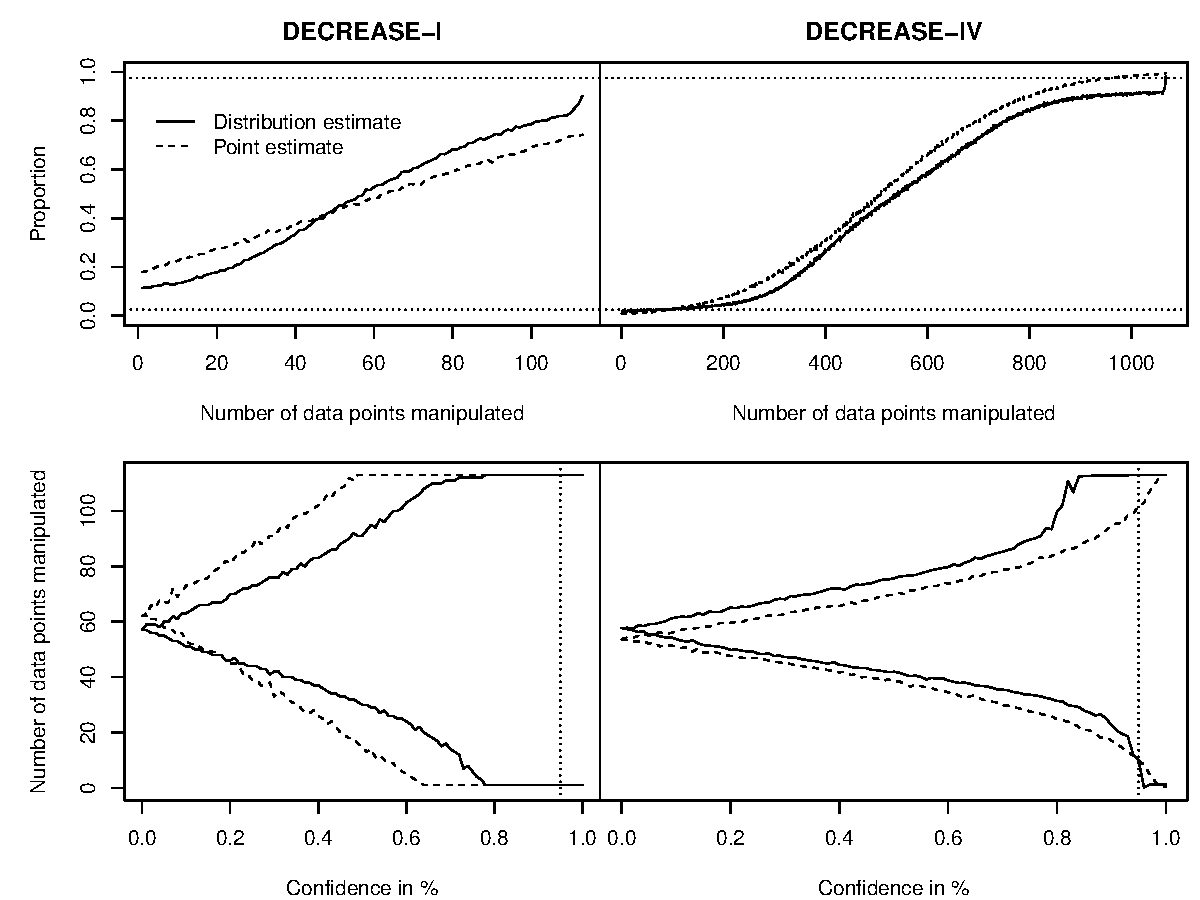
\includegraphics[width=0.8\linewidth]{../figures/fig3} 

}

\caption{Inversion method results used to estimate the number of data points manipulated in the DECREASE-I and DECREASE-IV trials. The top row panels indicate $p_M$ (y-axis) for all $X$ out of $N$ manipulated data points (x-axis). The bottom row indicates the estimated interval of manipulated data points (y-axis) when varying the degree of confidence (x-axis). Dotted lines indicate the bounds for a 95 percent CI.}\label{fig:figure 3}
\end{figure}

For DECREASE-IV (\(N=1066\)), the 95\% confidence interval for the
estimated number of manipulated data points is {[}3 - 1066{]} or {[}10 -
1066{]} when based on a point estimate or a more uncertain distribution
estimate, respectively. The relatively minor difference between the
estimates indicates that there is a high degree of confidence that data
manipulation did occur based on the difference of the trial results
alone. Nonetheless, the range of potentially manipulated data points is
still estimated at approximately 1000; this indicates that the summary
results are insufficient to provide more than an estimated lower bound.
This indicates that it is possible not all data were manipulated (i.e.,
\(N=1066\)), increasing the importance of well-documented data
provenance to discern between genuine and falsified data.

\section{Discussion}\label{discussion}

The effect of beta-blockade on perioperative mortality was already
unclear based on the investigations regarding scientific integrity; our
results strongly affirm that the empirical evidence from the DECREASE
trials is highly discrepant from other trials supposedly studying the
same effect (i.e., the effectiveness of beta-blockers in decreasing
perioperative mortality). Our results indicate that the results from the
DECREASE trials are nearly impossible to have arisen from the same
effect inspected by the non-DECREASE trials, except when we assume at
least some of the data were manipulated. As such, the scientific
validity of the DECREASE-I and DECREASE-IV trials should be regarded as
highly problematic and untrustworthy when assessing the effectiveness of
beta-blockade on perioperative mortality if they truly investigate the
same effects as the non-DECREASE trials, as is often
assumed\textsuperscript{9}. Nonetheless, the original papers that
presented these trial results are not yet
retracted\textsuperscript{2,3}, despite the integrity
reports\textsuperscript{4--6}.

Our approach to estimating the number of manipulated data points has one
major limitation that we would like to highlight: multiplicity. For each
estimated proportion of manipulated data points, there is another
smaller (or larger) proportion with more (or less) extremely manipulated
data points. This problem is similar to how various samples can give
rise to the same mean, but contain vastly different individual scores
within them (e.g., -2.5 and +2.5 versus -100 and +100; both give the
mean zero). Nonetheless, this limitation does still allow us to estimate
whether any data manipulation occurred because there is no multiplicity
in not manipulating data.

The ESC/ESA and ACC/AHA guidelines\textsuperscript{11,21} on
perioperative beta-blockade already excluded the DECREASE trials in
their assessment, but also state that other trials by Poldermans are
excluded. However, upon close inspection of the reference lists, the
ACC/AHA guidelines still cites four trials including Poldermans as
author as evidence for the guidelines\textsuperscript{2,22--24}, of
which two were already inspected by the scientific integrity committees
of Erasmus MC\textsuperscript{2,22}. In the ACC/AHA guidelines, the
following is said about studies conducted by Poldermans:

\begin{quote}
\emph{``If nonretracted DECREASE publications and/or other derivative
studies by Poldermans are relevant to the topic, they can only be cited
in the text with a comment about the finding compared with the current
recommendation but should not form the basis of that recommendation or
be used as a reference for the recommendation.''}\textsuperscript{11}
\end{quote}

Nonetheless, references are made without clear comments. Given the
confirmation of problems in the DECREASE-I and DECREASE-IV trials in our
results, it stresses that there is reason to distrust trials by
Poldermans. For the integrity of the guidelines and the safety of the
patients, we pose that investigations should be initiated into works
where Poldermans was involved and which were not cleared by the
scientific committees of Erasmus MC in their misconduct investigations.
Especially those papers cited as evidence in the ACC/AHA guidelines
should be investigated, considering that they affect patients and their
treatment directly.

Previously, further investigation of trials by Poldermans was deemed
unfeasible due to the lack of raw data; here we indicate methods that do
make it feasible. Based on just event-count data and trials that
supposedly investigate the same effect, we were able to estimate whether
part of the data were in fact manipulated and whether the results were
within reason of trials investigating the same effect. The results
clearly indicated they were not such reason.

The results of our analyses also highlight that, despite the lack of
availability of the raw data, summary results from larger samples allow
for better estimates of the number of manipulated data points when
similar trials are available. Moreover, larger trials result in
relatively more certainty (e.g., DECREASE-IV) about the estimated number
of manipulated data points, when using the inversion method, compared to
smaller trials (e.g., DECREASE-I). This increased certainty is due to
decreased standard errors of the estimated effects, resulting in higher
sensitivity to data anomalies. Nonetheless, much residual uncertainty
remains and simply less information is available in summary results when
compared to raw data. As such, raw data availability would improve the
options open to detect potential anomalies (note: raw data are available
for DECREASE VI, but upon a freedom of information request by the first
author, Erasmus MC refused to share these data; see
\href{https://osf.io/fswjt/}{osf.io/fswjt/}). The results also highlight
that in order to prevent detection, it would be in the manipulator's
interest to fabricate small and imprecise studies (assuming the
manipulator wants to remain undetected), which ultimately detracts from
the scientific value of such a study and hence the individual reward for
manipulation through reduced impact (hopefully).

With respect to clinical practice, the results provide some tentative
evidence that type of beta-blockade can severely influence perioperative
mortality. Our reanalysis of the Bouri et al.\textsuperscript{9} data
indicates that type of beta-blockade can reverse the effect on
perioperative mortality, even after taking into account whether a study
belongs to the DECREASE family. As such, atenolol seems to tentatively
decrease perioperative mortality, whereas the others (metoprolol,
propranolol, bisoprolol) increase perioperative mortality. However,
there seems to be covariation with respect to treatment administration,
duration, and dose, which further confounds whether the treatment effect
is due to type of beta-blocker or due to one of these other parameters.
There are too few studies (\(k=11\)) too properly discern the various
treatments from each other, requiring a new randomized trial with high
statistical power to determine moderating factors (if any). This affirms
the statement from the ESC/ESA guidelines that \emph{``high priority
needs to be given to new randomized clinical trials to better identify
which patients derive benefit from beta-blocker therapy in the
perioperative setting, and to determine the optimal method of
beta-blockade''}\textsuperscript{21}.

Moreover, the DECREASE and non-DECREASE trials seem to apply
beta-blockade from different conceptual viewpoints that could confound
the effectiveness of beta-blockade. The non-DECREASE trials seem to
focus purely on the application of beta-blockers in itself, whereas the
DECREASE trials use beta-blockade as a proxy to decrease resting heart
rate\textsuperscript{2,3}. As such, the DECREASE studies applied
beta-blockade at least a week in advance, specifically in order to lower
patient's resting heart rate to \textless{}70BPM and potentially
habituate the patient to the effects of the beta-blockade. Other studies
apply the beta-blockade just prior to the surgery (maximum: one day
prior) and therefore seem to regard the treatment specifically and not
the proxy of lowered BPM. As such, the differences between the DECREASE
and non-DECREASE trials might also in part be a consequence of the
different approaches in the various trials. Whether these differences
matter in treatment decisions is worthy of further research in a
clinical trial with high statistical power to find such differences.

In sum, our research indicates that the DECREASE trials are nearly
impossible if we assume they investigate exactly the same effect as the
non-DECREASE trials and under that assumption, our results provide some
evidence that at least some data points were manipulated. However, these
differences might also be due to different conceptual approaches as to
how beta-blockade might prevent mortality in non-cardiac surgery. We
recommend renewed investigations into Poldermans' work given these
findings --- especially those works still referenced by guidelines on
the use of beta-blockers without proper notice. Moreover, it remains
unclear whether beta-blockers might be effective in preventing mortality
rates in non-cardiac surgery patients. Considering this, we recommend
new and more extensively controlled, confirmatory trials to determine
whether there is any use in administering beta-blockers in order to
decrease perioperative mortality --- at the moment there is insufficient
evidence to determine any positive effect of beta-blockers on mortality
rates.

\section{Session info}\label{session-info}

\begin{verbatim}
## R version 3.4.0 (2017-04-21)
## Platform: x86_64-redhat-linux-gnu (64-bit)
## Running under: Fedora 25 (Workstation Edition)
## 
## Matrix products: default
## BLAS/LAPACK: /usr/lib64/R/lib/libRblas.so
## 
## locale:
##  [1] LC_CTYPE=en_US.UTF-8       LC_NUMERIC=C              
##  [3] LC_TIME=en_US.UTF-8        LC_COLLATE=en_US.UTF-8    
##  [5] LC_MONETARY=en_US.UTF-8    LC_MESSAGES=en_US.UTF-8   
##  [7] LC_PAPER=en_US.UTF-8       LC_NAME=C                 
##  [9] LC_ADDRESS=C               LC_TELEPHONE=C            
## [11] LC_MEASUREMENT=en_US.UTF-8 LC_IDENTIFICATION=C       
## 
## attached base packages:
## [1] stats     graphics  grDevices utils     datasets  methods   base     
## 
## other attached packages:
## [1] knitr_1.16      latex2exp_0.4.0 metafor_2.0-0   Matrix_1.2-9   
## 
## loaded via a namespace (and not attached):
##  [1] Rcpp_0.12.11    lattice_0.20-35 digest_0.6.12   rprojroot_1.2  
##  [5] grid_3.4.0      nlme_3.1-131    backports_1.1.0 magrittr_1.5   
##  [9] evaluate_0.10.1 highr_0.6       stringi_1.1.5   rmarkdown_1.6  
## [13] tools_3.4.0     stringr_1.2.0   yaml_2.1.14     compiler_3.4.0 
## [17] htmltools_0.3.6
\end{verbatim}

\section*{References}\label{references}
\addcontentsline{toc}{section}{References}

\hypertarget{refs}{}
\hypertarget{ref-Coleg5210}{}
1. Cole GD, Francis DP. Perioperative beta blockade: Guidelines do not
reflect the problems with the evidence from the decrease trials.
\emph{BMJ}. 2014;349.
doi:\href{https://doi.org/10.1136/bmj.g5210}{10.1136/bmj.g5210}.

\hypertarget{ref-poldermans1999}{}
2. Poldermans D, Boersma E, Bax JJ, et al. The effect of bisoprolol on
perioperative mortality and myocardial infarction in High-Risk patients
undergoing vascular surgery. \emph{The New England journal of medicine}.
1999;341(24):1789-1794.
doi:\href{https://doi.org/10.1056/NEJM199912093412402}{10.1056/NEJM199912093412402}.

\hypertarget{ref-dunkelgrun2009}{}
3. Dunkelgrun M, Boersma E, Schouten O, et al. Bisoprolol and
fluvastatin for the reduction of perioperative cardiac mortality and
myocardial infarction in intermediate-risk patients undergoing
noncardiovascular surgery: A randomized controlled trial (DECREASE-IV).
\emph{Annals of surgery}. 2009;249(6):921-926.
doi:\href{https://doi.org/10.1097/SLA.0b013e3181a77d00}{10.1097/SLA.0b013e3181a77d00}.

\hypertarget{ref-commissie2011}{}
4. Onderzoekscommissie Wetenschappelijke Integriteit. \emph{Onderzoek
Naar Mogelijke Schending van de Wetenschappelijke Integriteit: Beknopte
Versie}. Erasmus MC; 2011.
\url{https://web.archive.org/web/20151113121125/http://www.erasmusmc.nl/cs-research/bijlagen/integriteit/rapport-poldermans-2011}.

\hypertarget{ref-commissie2012}{}
5. Commissie Vervolgonderzoek 2012. \emph{Rapport Vervolgonderzoek Naar
Mogelijke Schending van de Wetenschappelijke Integriteit}. Erasmus MC;
2012.
\url{https://web.archive.org/web/20151027084205/http://www.erasmusmc.nl/5663/135857/3675250/3706798/erasmusmc.commissie.verv.onderzoek.2012}.

\hypertarget{ref-commissie2013}{}
6. Commissie Vervolgonderzoek Wetenschappelijke Integriteit 2013.
\emph{Rapport}. Erasmus MC; 2014.
\url{http://web.archive.org/web/20161104135848/http://www.erasmusmc.nl/cs-research/bijlagen/integriteit/eindrapport2014nl}.

\hypertarget{ref-Devereaux313}{}
7. Devereaux PJ, Beattie WS, Choi PT-L, et al. How strong is the
evidence for the use of perioperative beta blockers in non-cardiac
surgery? Systematic review and meta-analysis of randomised controlled
trials. \emph{BMJ}. 2005;331(7512):313-321.
doi:\href{https://doi.org/10.1136/bmj.38503.623646.8F}{10.1136/bmj.38503.623646.8F}.

\hypertarget{ref-Angeli2010}{}
8. Angeli F, Verdecchia P, Karthikeyan G, Mazzotta G, Gentile G, Reboldi
G. \(\beta\)-blockers reduce mortality in patients undergoing high-risk
non-cardiac surgery. \emph{American Journal of Cardiovascular Drugs}.
2010;10(4):247-259.
doi:\href{https://doi.org/10.2165/11539510-000000000-00000}{10.2165/11539510-000000000-00000}.

\hypertarget{ref-bouri2014}{}
9. Bouri S, Shun-Shin MJ, Cole GD, Mayet J, Francis DP. Meta-analysis of
secure randomised controlled trials of -blockade to prevent
perioperative death in non-cardiac surgery. \emph{Heart}.
2014;100(6):456-464.
doi:\href{https://doi.org/10.1136/heartjnl-2013-304262}{10.1136/heartjnl-2013-304262}.

\hypertarget{ref-esc2014}{}
10. ESC/ESA. Guidelines on non-cardiac surgery: Cardiovascular
assessment and management. \emph{European Heart Journal}.
2014;35:2383-2243.

\hypertarget{ref-Fleisher_2014}{}
11. Fleisher LA, Fleischmann KE, Auerbach AD, et al. 2014 ACC/AHA
guideline on perioperative cardiovascular evaluation and management of
patients undergoing noncardiac surgery: Executive summary: A report of
the american college of cardiology/american heart association task force
on practice guidelines. \emph{Circulation}. 2014;130(24):2215-2245.
doi:\href{https://doi.org/10.1161/cir.0000000000000105}{10.1161/cir.0000000000000105}.

\hypertarget{ref-Buyse1999-jq}{}
12. Buyse M, George SL, Evans S, et al. The role of biostatistics in the
prevention, detection and treatment of fraud in clinical trials.
\emph{Statistics in medicine}. 1999;18(24):3435-3451.
doi:\href{https://doi.org/10.1002/(SICI)1097-0258(19991230)18:24\%3C3435::AID-SIM365\%3E3.0.CO;2-O}{10.1002/(SICI)1097-0258(19991230)18:24\textless{}3435::AID-SIM365\textgreater{}3.0.CO;2-O}.

\hypertarget{ref-10.1111ux2fanae.13938}{}
13. Carlisle JB. Data fabrication and other reasons for non-random
sampling in 5087 randomised, controlled trials in anaesthetic and
general medical journals. \emph{Anaesthesia}. June 2017.
doi:\href{https://doi.org/10.1111/anae.13938}{10.1111/anae.13938}.

\hypertarget{ref-Knepper2016-la}{}
14. Knepper D, Lindblad AS, Sharma G, et al. Statistical monitoring in
clinical trials: Best practices for detecting data anomalies suggestive
of fabrication or misconduct. \emph{Therapeutic Innovation \& Regulatory
Science}. 4\textasciitilde{}feb 2016.
doi:\href{https://doi.org/10.1177/2168479016630576}{10.1177/2168479016630576}.

\hypertarget{ref-klei2015}{}
15. Klei W van. Welke perioperatieve bètablokker heeft de voorkeur?
{[}Which perioperative beta-blocker is preferred?{]}. \emph{Nederlands
Tijdschrift voor Geneeskunde}. 2015;159:A9798.

\hypertarget{ref-viechtbauer2010}{}
16. Viechtbauer W. Conducting meta-analyses in R with the metafor
package. \emph{Journal of Statistical Software}. 2010;36:1-48.
\url{http://www.jstatsoft.org/v36/i03/}.

\hypertarget{ref-viechtbauer2005}{}
17. Viechtbauer W. Bias and efficiency of meta-analytic variance
estimators in the Random-Effects model. \emph{Journal of educational and
behavioral statistics: a quarterly publication sponsored by the American
Educational Research Association and the American Statistical
Association}. 2005;30(3):261-293.
doi:\href{https://doi.org/10.3102/10769986030003261}{10.3102/10769986030003261}.

\hypertarget{ref-agresti2002}{}
18. Agresti A. \emph{Categorical Data Analysis}. Hoboken, NJ: John Wiley
\& Sons Inc.; 2002.

\hypertarget{ref-peters2015}{}
19. Peters CFW, Klaassen CAJ, Wiel MA van de. \emph{Evaluating the
Scientific Veracity of Publications by Dr. Jens Forster}. University of
Amsterdam; 2015.

\hypertarget{ref-casella2002}{}
20. Casella G, Berger RL. \emph{Statistical Interference}. Pacific
Grove, CA: Duxbury; 2002.

\hypertarget{ref-Kristensen_2014}{}
21. Kristensen SD, Knuuti J, Saraste A, et al. 2014 ESC/ESA guidelines
on non-cardiac surgery. \emph{European Journal of Anaesthesiology}.
2014;31(10):517-573.
doi:\href{https://doi.org/10.1097/eja.0000000000000150}{10.1097/eja.0000000000000150}.

\hypertarget{ref-Boersma_2001}{}
22. Boersma E, Poldermans D, Bax JJ, et al. Predictors of cardiac events
after major vascular surgery. \emph{JAMA}. 2001;285(14):1865.
doi:\href{https://doi.org/10.1001/jama.285.14.1865}{10.1001/jama.285.14.1865}.

\hypertarget{ref-van_Kuijk_2009}{}
23. Kuijk J-P van, Flu W-J, Schouten O, et al. Timing of noncardiac
surgery after coronary artery stenting with bare metal or drug-eluting
stents. \emph{The American Journal of Cardiology}.
2009;104(9):1229-1234.
doi:\href{https://doi.org/10.1016/j.amjcard.2009.06.038}{10.1016/j.amjcard.2009.06.038}.

\hypertarget{ref-Flu_2010}{}
24. Flu W-J, Kuijk J-P van, Chonchol M, et al. Timing of pre-operative
beta-blocker treatment in vascular surgery patients. \emph{Journal of
the American College of Cardiology}. 2010;56(23):1922-1929.
doi:\href{https://doi.org/10.1016/j.jacc.2010.05.056}{10.1016/j.jacc.2010.05.056}.


\end{document}
